\documentclass[12pt, A4]{report}
\usepackage[pdftex]{graphicx}
\usepackage[margin=1.2in]{geometry}
\usepackage[utf8]{inputenc}

\usepackage{graphicx}
\graphicspath{{./images/}}

\usepackage{listings}
\newcommand\lstinputpath[1]{\lstset{inputpath=#1}}
\lstinputpath{codes}

\usepackage{xcolor}
\usepackage{titlesec}
 
\titleformat{\chapter}[display]
  {\normalfont\bfseries}{}{0pt}{\Huge}

\definecolor{codegreen}{rgb}{0,0.6,0}
\definecolor{codegray}{rgb}{0.5,0.5,0.5}
\definecolor{codepurple}{rgb}{0.58,0,0.82}
\definecolor{backcolour}{rgb}{0.95,0.95,0.92}

\lstdefinestyle{mystyle}{
    backgroundcolor=\color{backcolour},   
    commentstyle=\color{codegreen},
    keywordstyle=\color{magenta},
    numberstyle=\tiny\color{codegray},
    stringstyle=\color{codepurple},
    basicstyle=\ttfamily\footnotesize,
    breakatwhitespace=false,         
    breaklines=true,                 
    captionpos=b,                    
    keepspaces=true,                 
    numbers=left,                    
    numbersep=5pt,                  
    showspaces=false,                
    showstringspaces=false,
    showtabs=false,                  
    tabsize=2
}

\lstset{style=mystyle}

\usepackage{hyperref}
\hypersetup{
    colorlinks=true,
    linkcolor=blue,
    filecolor=magenta,      
    urlcolor=cyan,
}

\urlstyle{same}


\title{\textbf{Neural Network and Machine Learning}\\\large{Midterm Report for Summer of Science - 2020}}
\author{Name: Sahasra Ranjan\\Mentor: Amitrajit Bhattacharjee}
\date{Roll no.: 190050102}

\begin{document}

\begin{titlepage}
\maketitle
\tableofcontents{}
\end{titlepage}

Machine Learning is undeniably one of the most influential and powerful technologies in today’s world. It is a tool for turning information into knowledge. In the past 50 years, there has been an explosion of data. This mass of data is useless unless we analyse it and find the patterns hidden within. Machine learning techniques are used to automatically find the valuable underlying patterns within complex data that we would otherwise struggle to discover. The hidden patterns and knowledge about a problem can be used to predict future events and perform all kinds of complex decision making.\\\\
There are multiple forms of Machine Learning; supervised, unsupervised , semi-supervised and reinforcement learning. Each form of Machine Learning has differing approaches, but they all follow the same underlying process and theory. I'll cover supervised and unsupervised learning for my report.

\section{Supervised and Unsupervised Learning}
  The most basic thing to remember is that we already know what our correct output should look like in Supervised Learning.
  But, we have little or no idea about what our results should look like.\\

  \textbf{Supervised Learning:}
  \begin{itemize}
    \item Classification: Spam/Not-spam. 
    \item Regression: Predicting age.
  \end{itemize}

  \textbf{Unsupervised Learning:}
  \begin{itemize}
    \item Clustering: Grouping based on different variables.
    \item Non Clustering: Finding structue in chaotic environment.
  \end{itemize}

\chapter{Linear Regression}
  Regression being a part of Supervised Learning is used for estimating data with real-valued output.  

  \subsection{Cost Function}
    This function measures the performance of a Machine Learning model for given data.

    \textbf{Hypothesis}: $ h_ \theta(x) = \theta_0 + \theta_1x $

    \textbf{Parameters:} $ \theta_0, \theta_1 $

    \textbf{Cost Function:} 
    \begin{equation} \label {eq:1}
        J( \theta_0, \theta_1 ) = 1/2m \sum_{i=1}^{m} (h_\theta(x^{(i)})-y^{(i)})^2 
    \end{equation} 

    \textbf{Goal:} Minimize cost function with $ \theta_0, \theta_1 $ as parameters.

  \subsection{Gradient Descent}

    \textbf{Basic idea:}
    \begin{itemize}
    \item Start with some $ \theta_0, \theta_1 $
    \item Keep changing $ \theta_0, \theta_1 $ to reduce $ J(\theta_0, \theta_1) $ until we end up at minima.
    \end{itemize} 

    \textbf{Algorithm:}
     repeat until convergence:
    \begin{equation} \label {eq:2}
        \theta_j := \theta_j - \alpha \frac{\partial {J(\theta_0, \theta_1)}}{\partial \theta_j}
    \end{equation} 

    (for  $j = 0, 1 $  ,here).  

    \textbf{Intution:} 
    If $\alpha$ is too small, the descent can be slow and if too large, descent may fail to converge or even diverge.
    Gradient descent can converge to a local minimum, even with a fixed learning rate $\alpha$. As we approach local minimum, gradient descent will automatically take smaller steps. So, no need to decrease $\alpha$ over time. 

  \subsection{Gradient Descent for linear regression}
    Combining gradient descent algorithm with linear regression model, we get:

    \begin{equation} \label {eq:3}
        j = 0 : \frac{\partial {J(\theta_0, \theta_1)}}{\partial \theta_0} = 1/2 \sum_{i=1}^{m} (h_\theta(x^{(i)})-y^{(i)}) 
    \end{equation}

    \begin{equation} \label {eq:4}
        j = 1 : \frac{\partial {J(\theta_0, \theta_1)}}{\partial \theta_1} = 1/2 \sum_{i=1}^{m} (h_\theta(x^{(i)})-y^{(i)}).x^{(i)}
    \end{equation}

    Now, we can repeat \ref{eq:3} and \ref{eq:4} until convergence to obtain the minima.

    "Batch" gradient descent: Each step of gradient descent uses all the training examples.
    For eq. "m" batches in equation \ref{eq:1}.


\section{Multivariate Linear Regression}
  Linear regression involving more than one variable. For eq., Predicting the price of a house based on parameters "Plot Area", "No. of Floors", "Connectivity with markets", etc.

  \subsection{Multiple Features}
    The multivariable form of the hypothesis is as follows:
    \begin{equation} \label {eq:5}
        h_\theta(x) = \theta_0 + \theta_1x_1 + \theta_2x_2 + \theta_ 3x_3 + ... + \theta_{n}x_n.    
    \end{equation}
    This hypothesis funtion can be concisely represented as:
    \begin{equation}
        h_\theta(x) = \theta^{T}x
    \end{equation}
    where, $ \theta^T $ is a 1xn matrix consisting of $ \theta_0, \theta_1, \theta_2 ... \theta_n $.


  \subsection{Gradient Descent for Multiple Variables}
    Gradient descent formula for Multiple variables will be similar to that of a single variable.

    \begin{equation} \label {eq: GD for multiple}
        \theta_j =  \theta_j - \alpha \frac{1}{m} \sum_{i=1}^{m} (h_\theta(x^{(i)})-y^{(i)}).x_j^{(i)}
    \end{equation}

    Repeating this equation until convergence will give the minima. \footnote[1]{$x_0 = 1$ in equation \ref{eq: GD for multiple}}

  \subsubsection{Feature Scaling}
    Feature Scaling is used to reduce the number of iterations in Gradient Descent.The basic idea of feature scaling is to bring all the features on the same scale. (in general we try to approximate every feature in the range $ -1 < x_i < 1 $)
    \\ \\ Reducing the number of iteration doesn't mean making computation of each step easier. And also it does not affect computational efficiency of Normal Equation.

  \subsubsection{Mean Normalisation}
    Mean Normalisation makes features to have approximately zero mean.

  \subsubsection{Learning Rate}
    If $\alpha$ is too small: slow convergence.\\ \\
    if $\alpha$ is too large: $J(\theta)$ may not decrease on every iteration, or may not converge.

  \subsubsection{Polynomial Regression}
    Selecting proper polynomial for fitting data is very important.

    \begin{figure}[h]
        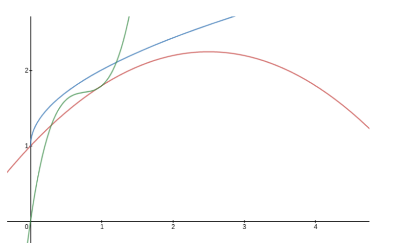
\includegraphics[scale = 0.6]{polyreg.png}
    \end{figure}

    \textbf{Red:} Quadratic

    \textbf {Blue:} Square root funtion $ \theta_0+\theta_1x+\theta_2\sqrt{x} $

    \textbf {Green:} Cubic function
\\ \\

\section{Normal equation}
  Normal Equation is a method to solve for $\theta_T$ analytically, by creating a $m\times(n+1)$ matrix $X$ and another $m\times1$ matrix $Y$.\footnote[2]{Every element of first column of matrix $X$ is 1 and other are the feature's coefficient}

  Mathematically $\theta$ is given as:
  \begin{equation} \label {eq: theta}
    \theta = (X^TX)^{-1}X^ty
  \end{equation}

  \begin{tabular}{ |c|c|}
    \hline
    \textbf{Gradient Descent} & \textbf{Normal Equation} \\
    \hline
    Need to choose $\alpha$ & No need to choose $\alpha$ \\
    Needs many iteration & Don't need to iterate \\
    Works well with large n & Slow for large n \\
    \hline
  \end{tabular}

  \vspace{5mm}

  \subsubsection{Reasons for non-invertiblity of $X^T X$}
    \begin{itemize}
        \item Redundant features (linear dependence) \footnote[3]{Eg. Using both $m^2 \  \& \  (feet)^2$ features}
        \item Too many features (m $<=$ n) 
    \end{itemize}

\section{Classification and Represention}


  \subsection{Classification}
    The classification problem is just like the regression problem, except that the values we now want to predict take on only a small number of discrete values. For now, we'll discuss the binary classification problem.

  \subsection{Hypothesis Representation}
    We may use out old regression algorithm by classifying data on the basis of a threshold. But it will have very poor performance.\\ 
    \\We will introduce "Sigmoid Function", also called the "Logistic Function":
    \begin{equation}
      h_\theta(x) = g(\theta^{T}x)
    \end{equation}
    \begin{equation}
      z = \theta^{T}x
    \end{equation}
    \begin{equation}\label{eq:sigmoid}
      g(z) = \frac{1}{1+e^{-z}}
    \end{equation}
    This is how the Sigmoid Function looks like:
    \begin{figure}[h]
      \centering
      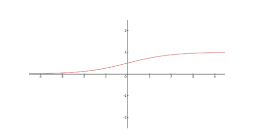
\includegraphics[scale = 1]{sigmoid.png}
      \caption{Sigmoid Funtion \ref{eq:sigmoid}}
    \end{figure}

  \subsection{Decision Boundary}
    The decision boundary is the line that separates the area where y=0 and where y=1.\\
    It is similar to the decision boundary for linear regression, the only difference is distribution of values (linear and sigmoid)

  \subsection{Worked-out Example}
	\lstinputlisting[language=Octave, caption=Octave Implementation for Linear Regression Algorithms]{linearRegression.m}

\chapter{Logistic Regression}

  \subsection{Cost Function}
    Cost funtion for logistic regression looks like:

    \begin{equation}
      J(\theta) = \frac{1}{m}\sum_{i=1}^{m}Cost(h_\theta(x^{(i)}), y^{(i)})
    \end{equation}
    \\ \\
    $ Cost(h_\theta(x),y) = -\log{(h_\theta{(x)})} $ \hfill if $y = 1$
    \\ \\
    $Cost(h_\theta(x),y) = -\log{(1-h_\theta{(x)})}$  \hfill if $y = 0$

    \begin{figure}[h]
      \centering
      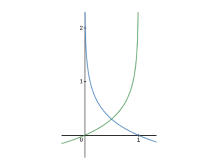
\includegraphics[scale = 0.75]{costlog.png}
      \caption{Cost Funtion}
    \end{figure}

    \subsubsection{Siplified Cost Funtion}
    This cost funtion can be compressed into a single funtion:
    \begin{equation}
      Cost(h_\theta(x),y) = -y\log{(h_\theta{(x)})} -(1-y)\log{(1-h_\theta{(x)})}
    \end{equation}
    A vectorised implementation is: \\ \\
    $h = g(X\theta)$\\
    $J(\theta) = \frac{1}{m}.(-y^T\log{h}-(1-y)^T\log{1-h})$
    \\ \\
    Vectorised implementation for Gradient Descent: \\ \\
    $\theta := \theta - \frac{\alpha}{m}X^T(g(X\theta)-y)$

\section{Multiclass Classification}
  \subsection{One-vs-all}
    This approach is when data has more than two categories.We divide our problem into n\footnote[1]{n = no of categories in dataset} binary classification problems, in each one, we predict the probability considering one of the category to be $+$ve and all other to be $-$ve. Repeating this for all other categories will finally give us all the decision boundaries.
    \begin{figure}[h]
      \centering
      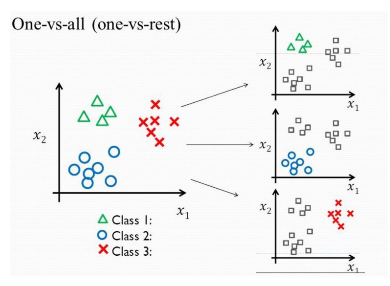
\includegraphics[scale = 0.6]{oneall.png}
      \caption{One vs all classifiaction method}
    \end{figure}   

  \subsection{Worked-out Example}
	\lstinputlisting[language=Octave, caption=Octave Implementation for Logistic Regression Algorithms]{logisticRegression.m}


\chapter{Decision Tree}
\documentclass[12pt, A4]{report}
\usepackage[utf8]{inputenc}

\usepackage{graphicx}
\graphicspath{{./images/}}

\usepackage{listings}
\usepackage{xcolor}

\definecolor{codegreen}{rgb}{0,0.6,0}
\definecolor{codegray}{rgb}{0.5,0.5,0.5}
\definecolor{codepurple}{rgb}{0.58,0,0.82}
\definecolor{backcolour}{rgb}{0.95,0.95,0.92}

\lstdefinestyle{mystyle}{
    backgroundcolor=\color{backcolour},   
    commentstyle=\color{codegreen},
    keywordstyle=\color{magenta},
    numberstyle=\tiny\color{codegray},
    stringstyle=\color{codepurple},
    basicstyle=\ttfamily\footnotesize,
    breakatwhitespace=false,         
    breaklines=true,                 
    captionpos=b,                    
    keepspaces=true,                 
    numbers=left,                    
    numbersep=5pt,                  
    showspaces=false,                
    showstringspaces=false,
    showtabs=false,                  
    tabsize=2
}

\lstset{style=mystyle}

\usepackage{hyperref}
\hypersetup{
    colorlinks=true,
    linkcolor=blue,
    filecolor=magenta,      
    urlcolor=cyan,
}

\urlstyle{same}


\title{\textbf{Decision Tree}\\ \large{Supervised ML Algorithm}}
\author{Sahasra Ranjan}
\date{April 2020}

\begin{document}

\begin{titlepage}
\maketitle
\end{titlepage}

A decision tree is a map of the possible outcomes of a series of a related choices. It allows to weigh possible actions against one another based of various factors.\par
It uses a tree-like model of decision. It typically starts with a single node, which branches into possible outcomes. Each of those outcomes leads to additional nodes, which branch off into other possiblities. 

\begin{figure}[h]
	\centering
	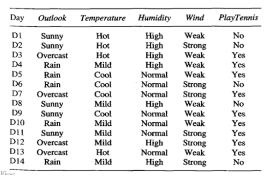
\includegraphics[width=6cm, height=4cm]{dtdata1.png}
	\caption{Dataset for possiblity of a tennis match}
	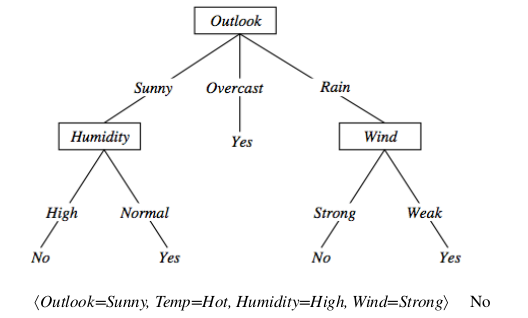
\includegraphics[width=8cm, height=5cm]{dtdata2.png}
	\caption{Decision Tree for the same}
\end{figure}

\subsection*{Advantages and Disadvantages of Decision Trees}
	\textbf{Advantages:}
	\begin{itemize}
		\item Performs classification without requiring much computation.
		\item Provides clear indication of important fields for prediction of classification.
	\end{itemize}
	\vspace{15mm}
	\textbf{Disadvantages:}
	\begin{itemize}
		\item Less appropriate for predicting continious attributes.
		\item Computationally expensive to train
	\end{itemize}

\vspace{5mm}
\subsection*{Creating a Decision Tree}
	For every node, we have to create subtrees with all the possiblities. and then further repeat for other features.\par
	For eg., In the tennis match problem, for the first node  let's check outlook, since having three possiblity (viz. Sunny, Overcast, Rainy), we created three subtrees and then further we keep asking for other features like Humidity \& wind to get the final tree.  

\vspace{5mm}
\subsection*{Greedy Approach for creating decision tree}
	Greedy approach is implemented by making an optimal local choice at each node. By making these local optimal choices, we reach the approximate optimal solution globaly.

	The algorithm can be summarized as: 
	\begin{enumerate}
		\item At each stage (node), pick out the best feature as the test conditiion.
		\item Now split the node into possibel outcomes (internal nodes)
		\item Repeat the above steps till all the test conditions have been exhausted into leaf nodes.
	\end{enumerate}

\vspace{5mm}
\subsection*{Continuous Features}
	There might be some feature which are not categorical, for these we need to create possibilities on the basis of aprropriate ranges. One such tree is shown below:
	\begin{figure}[h]
		\centering
		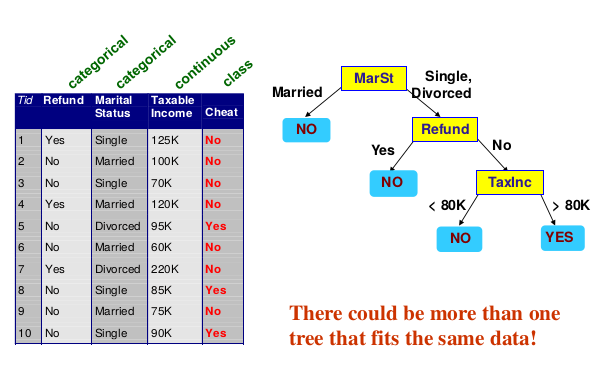
\includegraphics[width=12cm, height=6cm]{continuousDT.png}
		\caption{Decision tree with continuous feature}
	\end{figure}


\subsection*{Entropy}
	In the most layman terms, Entropy is nothing but the \textbf{The measure of disorder}.
	Why is it important to study entropy for machine learning? \\
	\\ Entropy is a measure of disorder or uncertainity and the goal of machine learning models and Data Scientists in general is to reduce uncertainity.\\
	\\ The Mathematical formula for entropy is - 
	\begin{equation}\label {eq:entropy}
		E(S) = \sum_{i=1}^c - p_i log_2 p_i\
	\end{equation}
	Where $p_i$ is the frequentist probability of an element/class $i$ in out data.\\
	\\ Let's say we have only two classes, a positive and a negative class. Out of 100 data, suppose that 70 belongs to $-$ve class and 30 to $+$ve. Then, P$+$ will be 0.3 and P$-$ will be 0.7.
	\vspace{4mm}
	Entropy $E$ will be given by:
	\begin{equation}
		E = -\frac{3}{10} \times log_2{\frac{3}{10}}-\frac{7}{10} \times log_2{\frac{7}{10}} \approx \textbf{0.88}
	\end{equation}
	\begin{figure}[h]
		\centering
		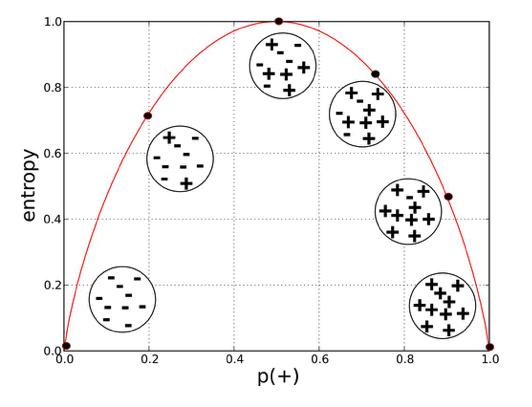
\includegraphics[width=8cm, height=6cm]{entropyDT.png}
		\caption{Entropy distribution frequentist probability}
	\end{figure}

\subsection*{Information Gain}
	Information gain is basically how much Entropy is removed after training a decision tree.\\
	\textbf{Higher information gain = more entropy removed.}\\
	In technical terms, Information Gain from X on Y is defined as:
	\begin{equation}\label{eq:inforamtion gain}
		IG(Y,X) = E(Y) - E(Y|X)
	\end{equation}
	Basics of inforation gain is well explained here: \href{https://victorzhou.com/blog/information-gain/}{A Simple Explanation of Information Gain and Entropy}

\subsection*{Example: Decision Tree}
	Consider an example where we are building a decision tree to predict whether a loan given to a person would result in a write-off or not. Our entire population consists of 30 instances. 16 belong to the write-off class and the other 14 belong to the non-write-off class. We have two features, namely “Balance” that can take on two values: “$<$ 50K” or “$>$ 50K” and “Residence” that can take on three values: “OWN”, “RENT” or “OTHER”. I’m going to show you how a decision tree algorithm would decide what attribute to split on first and what feature provides more information, or reduces more uncertainty about our target variable out of the two using the concepts of Entropy and Information Gain.
	\begin{figure}[h]
		\centering
		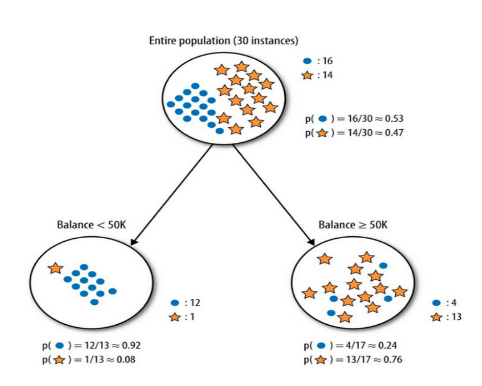
\includegraphics[width=10cm, height=7.5cm]{tree1.png}
		\caption{Feature 1: Balance}
	\end{figure}
	The dots are the data points with class right-off and the stars are the non-write-offs. Splitting the parent node on attribute balance gives us 2 child nodes. The left node gets 13 of the total observations with 12/13 ( 0.92 probability) observations from the write-off class and only 1/13( 0.08 probability) observations from the non-write of class. The right node gets 17 of the total observation with 13/17( 0.76 probability) observations from the non-write-off class and 4/17 ( 0.24 probability) from the write-off class.
	\\ \\Let’s calculate\footnote[1]{See this for calculations and further refrences: \href{https://towardsdatascience.com/entropy-how-decision-trees-make-decisions-2946b9c18c8}{Entropy: How Decision Trees Make Decisions}} the entropy for the parent node and see how much uncertainty the tree can reduce by splitting on Balance.	
	Splitting on feature ,“Balance” leads to an information gain of 0.37 on our target variable. Let’s do the same thing for feature, “Residence” to see how it compares.\\ 
	\begin{figure}[h]
		\centering
		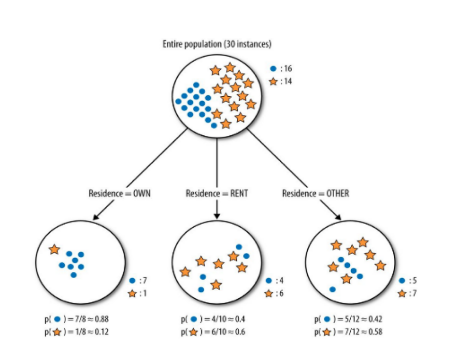
\includegraphics[width=10cm, height=7.5cm]{tree2.png}
		\caption{Feature 2: Residence}
	\end{figure}
	\\
	Splitting the tree on Residence gives us 3 child nodes. The left child node gets 8 of the total observations with 7/8 (0.88 probability) observations from the write-off class and only 1/8 (0.12 probability) observations from the non-write-off class. The middle child nodes gets 10 of the total observations with 4/10 (0.4 probability) observations of the write-off class and 6/10( 0.6 probability) observations from the non-write-off class. The right child node gets 12 of the total observations with 5/12 ( 0.42 probability) observations from the write-off class and 7/12 ( 0.58 ) observations from the non-write-off class. We already know the entropy for the parent node. We simply need to calculate the entropy after the split to compute the information gain from “Residence”

	The information gain from feature, Balance is almost 3 times more than the information gain from Residence! If you go back and take a look at the graphs you can see that the child nodes from splitting on Balance do seem purer than those of Residence. However the left most node for residence is also very pure but this is where the weighted averages come in play. Even though that node is very pure, it has the least amount of the total observations and a result contributes a small portion of it’s purity when we calculate the total entropy from splitting on Residence. This is important because we’re looking for overall informative power of a feature and we don’t want our results to be skewed by a rare value in a feature.
	\\ \\
	By itself the feature, Balance provides more information about our target variable than Residence. It reduces more disorder in our target variable. A decision tree algorithm would use this result to make the first split on our data using Balance. From here on, the decision tree algorithm would use this process at every split to decide what feature it is going to split on next. In a real world scenario , with more than two features the first split is made on the most informative feature and then at every split the information gain for each additional feature needs to be recomputed because it would not be the same as the information gain from each feature by itself. The entropy and information gain would have to be calculated after one or more splits have already been made which would change the results. A decision tree would repeat this process as it grows deeper and deeper till either it reaches a pre-defined depth or no additional split can result in a higher information gain beyond a certain threshold which can also usually be specified as a hyper-parameter!
	\\ \\
	There you have it! You now know what entropy and information gain are and how they are computed. You understand how a decision tree either by itself or in a tree based ensemble decides on the best order of features to split on and decides when to stop when it trains itself on given data. If you every have to explain the intricacies of how decision trees work to someone, hopefully you won’t do too bad.\\

\subsection*{Implementation}
\lstinputlisting[language=Octave, caption=Python Implementation for Decision Tree]{dtScratch.py}

\end{document}

\chapter{Naive Bayes}
\section*{Naive Bayes}

Naive Bayes methods are a set of supervised learning algorithms based on applying Bayes' theorem with the "naive" assumption of conditional independence between every pair of features given the value of the class variable.\\ \\
What actually Bayes' theorem is?
\begin{equation}\label {eq:bayes}
    P(A|B) = \frac{P(B|A)P(A)}{P(B)}
\end{equation}
$P(A|B)$ is the probability of \textbf{A} happening, given that \textbf{B} has occured.\\ \\ Why "Naive"? Because the presence of one particular feature does not affect the other.
\\ \\ 
Without going to deep, let's see an example:

\subsection*{The Golf Match Problem}
    Consider the problem of playing golf, dataset for the same:
    \begin{figure}[h]
        \centering
        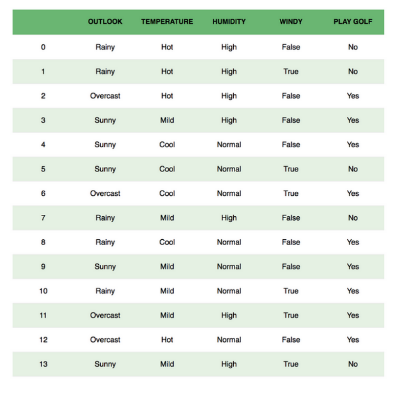
\includegraphics[scale=0.7]{golf.png}
        \caption{Dataset for possiblity of a golf match}
    \end{figure}

    Bayes theorem for this example can be rewritten as:
    \begin{equation}
        P(y|X) = \frac{P(X|y)P(y)}{P(X)}
    \end{equation}

    The variable \textbf{y} is the class variable (play golf), which represents if it is suitable to play golf or not given the conditions. Variable \textbf{X} is a matrix representing the parameters/features.
    \\ \\
    $\textbf{X} = (x_1, x_2, x_3, ... , x_n)$ \hfill    \small{$x_1, x_2, ... x_n$ represent the features}\footnote[1]{temperature, humidity and windy (here)}.
    \\ \\

    \begin{equation}
        P(y|x_1, ..., x_n) = \frac{P(x_1|y)P(x_2|y)...P(x_n|y)P(y)}{P(x_1)P(x_2)...P(x_n)}
    \end{equation}
    These values can be obtained by looking at the dataset and substituting them into the equation will give us the result.
    \\ \\
    In our case, the the class variable(\textbf{y}) has only two outcomes, yes or no. Therefore, we need to find class \textbf{y} with maximum probability. 
    \begin{equation}
        y = argmax_yP(y)\prod_{i=1}^{n}P(x_i|y)
    \end{equation}

\subsection*{Types of Naive Bayes classifier:}
    \subsubsection*{Miltinomial Naive Bayes:}
        This is mostly used for the document classification problem, i.e whether a document belongs to the category of sports, politics, technology etc. The features/predictors used by the classifier are the frequency of the words present in the document.

    \subsubsection*{Bernoulli Naive Bayes}
        This is similar to the multinomial Naive Bayes but the predictors are boolean variables. The parameters that we use to predict the class variable take up only values yes or no, for example, if a word occurs in the text or not.

    \subsubsection*{Gaussian Naive Bayes}
        When the predictors take up a continuous value and are not discrete, we assume that these values are sampled from a gaussian distribution.

        \begin{figure}[h]
            \centering
            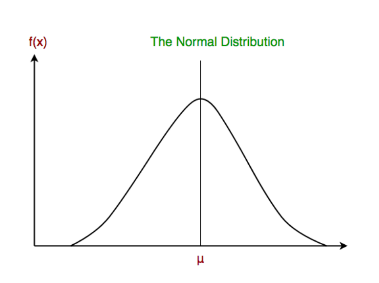
\includegraphics[scale=0.6]{gaussiannaive.png}
            \caption{Gaussian Distribution(Normal Distribution)}
        \end{figure}

        The formula for conditional probability changes to:

        \begin{equation}
            P(x_i|y) = \frac{1}{\sqrt{2\pi\sigma_y^2}}e^{-\frac{(x_i-\mu_y)^2}{2\sigma_y^2}}
        \end{equation}

\subsection*{Laplace Smoothing}
    It is problematic when a frequency-based probability is zero because it will wipe out all the information in the other probabilities.\\ \\
    A solution would be \textbf{Laplace smoothing}, which is a technique for smoothing categorical data. A small-sample correction, or \textbf{pseudo-count}, will be incorporated in every probability estimate. Consequently, no probability will be zero. this is a way of regularizing Naive Bayes, and when the pseudo-count is zero, it is called Laplace smoothing. While in the general case it is often called \textbf{Lidstone smoothing.}

    \begin{equation}
        P_{i,\ \alpha-smoothed} = \frac{x_i+\alpha}{N+\alpha d}
    \end{equation}
    where, $\alpha > 0$ the "pseudocount" is a smoothing parameter. And, $1/d$ is the \href{https://en.wikipedia.org/wiki/Discrete_uniform_distribution}{Uniform Probability}.

    \subsubsection*{Note}
    In practice, we use logs to represent probabilities:
    \begin{equation}
        \log{(P(x_1|y)P(x_2|y)...P(x_n|y))} = \log{P(x_1|y)} + \log{P(x_2|y)} +...+ \log{P(x_n|y)}
    \end{equation}


\subsection*{Applications}
    Naive Bayes algorithms are mostly used in sentiment analysis, spam filtering, recommendation systems etc. They are fast and easy to implement but their biggest disadvantage is that the requirement of predictors to be independent. In most of the real-life cases, the predictors are dependent, this hinders the performance of the classifier.

\subsection*{Worked-out Implementation\footnote[2]{ \textbf{Output:}\\
23 columns, after dropping NA, 22\\
Test 1\\
5671 correct of 5687\\
Accuracy: 0.997186565851943\\
Test 2\\
2433 correct of 2437\\
Accuracy: 0.9983586376692655\\ 
\\This implementation of Naive Bayes Algorithm has an accuracy of approximately 99.8\% which is good in the first go.}}
\lstinputlisting[language=Python, caption=Python Implementation for Naive Bayes]{naiveBayes-implementation.py}


\chapter{k-Nearest Neighbours}
\input{sections/KNN}

\chapter{Neural Networks}
  At a very simple level, neurons are basically computational units that take inputs (\textbf{dendrites}) as electrical inputs (called "spikes") that are channeled to outputs (\textbf{axons}). In our model, our dendrites are like the input features $x_1...x_n$, and the output is the result of our hypothesis function. In this model our $x_0$ input node is sometimes called the "bias unit." It is always equal to 1.

  \begin{figure}[h]
    \centering
    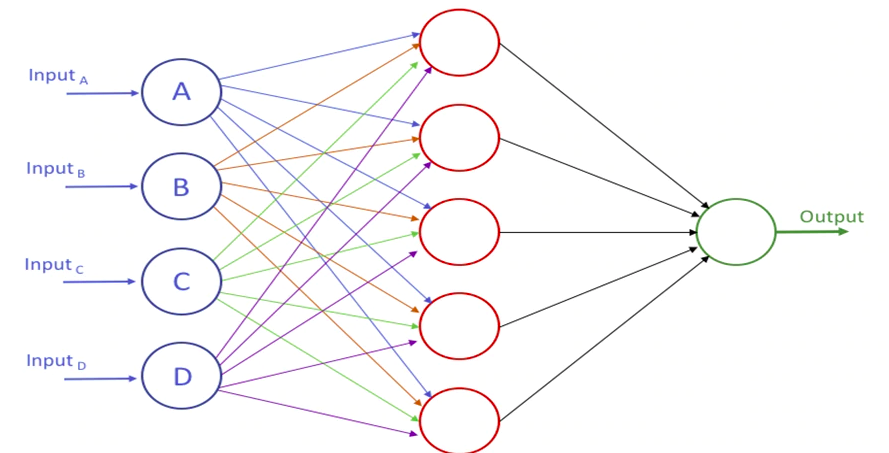
\includegraphics[scale=0.3]{neuralnetwork.png}
  \end{figure}

  Our input nodes (layer 1), also known as the "input layer", go into another node (layer 2), which finally outputs the hypothesis function, known as the "output layer". We can have intermediate layers of nodes between the input and output layers called the "hidden layers."
  \\\\
  These "hidden layer" nodes are called as "activation units". The values for each activation nodes are represented as: \\
  \begin{figure}[h]
    \centering
    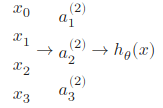
\includegraphics[scale=0.6]{hiddenlayer.png}
  \end{figure}

  \begin{equation}
    a_1^{(2)} = g(\theta_{10}^{(1)}x_0 + \theta_{11}^{(1)}x_1 + \theta_{12}^{(1)}x_2 + \theta_{13}^{(1)}x_3)
  \end{equation}
  \begin{equation}
    a_2^{(2)} = g(\theta_{20}^{(1)}x_0 + \theta_{21}^{(1)}x_1 + \theta_{22}^{(1)}x_2 + \theta_{23}^{(1)}x_3)
  \end{equation}
  \begin{equation}
    a_3^{(2)} = g(\theta_{30}^{(1)}x_0 + \theta_{31}^{(1)}x_1 + \theta_{32}^{(1)}x_2 + \theta_{33}^{(1)}x_3)
  \end{equation}
  \begin{equation}
    h_\theta(x) = a_1^{(3)]} = a_1^{(2)} = g(\theta_{10}^{(2)}x_0 + \theta_{11}^{(2)}x_1 + \theta_{12}^{(2)}x_2 + \theta_{13}^{(2)}x_3)5
  \end{equation}
  \\From these equations, we can conclude that we will get a matrix for each layer to calculate the weight for the second layer.

  \section{Intutions}
    \subsection{OR Function}
      \begin{figure}[h]
        \centering
        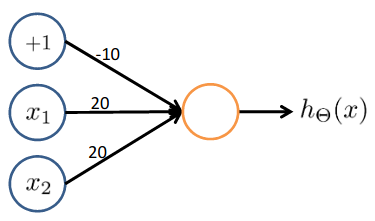
\includegraphics[scale=0.5]{ornet.png}
        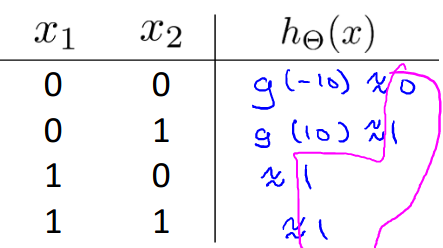
\includegraphics[scale=0.4]{ortable.png}
      \end{figure}

    \subsection{Important Note}
      \begin{figure}[h]
        \centering
        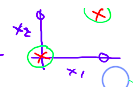
\includegraphics[scale=1]{important-net.png}
      \end{figure}

      For any prediction which involves a straight line as decision boundary, we can represent it with a neural network without any hidden layer but otherwise, we'll have to include few hidden layers. An important point to note is that we can represent almost any distribution with a certain arrangement of Neural Network.

  \section{Multiclass Classification}
    To classify data into multiple classes, we'll have to define out set of resulting classes as y:
    \begin{figure}[h]
      \centering
      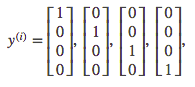
\includegraphics[scale=0.6]{resultnet.png}
    \end{figure}

  \section{Cost Function}
    Let's first define a few variables that we'll need to use:
    
    \begin{itemize}
      \item L = total number of layers in the network
      \item numbers of units (non counting bias unit) in layer 1
      \item K = numbet of output unit/classes
    \end{itemize}

    The cost function for neural networks will be slightly more complicated as it involves a few other factors of 'K' and 'L' defined earlier.

    \begin{equation}
      J(\theta) = -\frac{1}{m}\sum_{i=1}^{m}\sum_{k=1}^{K}y_k^{(i)}\log((h_\theta(x^{(i)}))_k) + (1-y_k^{(i)})\log(1-(h_\theta(x^{(i)}))_k) + \frac{\lambda}{2m}\sum_{l=1}^{L-1}\sum_{i=1}^{s_l}\sum_{j=1}^{s_{l+1}} (\theta_{j,i}^{(L)})^2
    \end{equation}

    \textbf{Note:}
    \begin{itemize}
      \item the double sum simply adds up the logistic regression costs calculated for each cell in the output layer.
      \item the triple sum simply adds up the squares of all the individual $\theta$s in the entire network.
      \item the I in the triple sum does not refer to training example i.
    \end{itemize}

  \section{Backpropagation Algorithm}
    Given training set ${(x^(1),y^(1))...(x^(m),y^(m))}$
    \begin{itemize}
      \item Set $\Delta^{(l)}_{i,j} := 0$ for all (l,i,j), (hence you end up having a matrix full of zeros)
    \end{itemize}

    For training example t=1 to m:
    \begin{enumerate}
      \item Set $a^{(1)} := x^{(t)}$
      \item Perform forward propagation to compute $a^{(l)}$ for l = 2,3,...,L

      \textbf{Gradient Computation}

      \item Using $y^{(t)}$, compute $\delta^{(L)} = a^{(L)} - y^{(L)}$
      \item Compute $\delta^{(l)}$
      \item $\Delta^{(L)} := \Delta^{(L)} + \delta^{(l+1)}(a^{(l)})^T$

      \begin{figure}[h]
        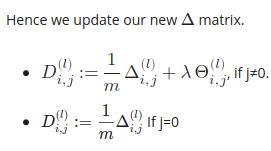
\includegraphics[scale=0.65]{bpupdate.png}
      \end{figure}
    \end{enumerate}

  \section{Gradient Checking}
    Gradient checking will assure that our backpropagation works as intended. We can approximate the derivative of our cost function with:

    \begin{figure}[h]
      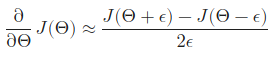
\includegraphics[scale=0.65]{gc.png}
    \end{figure}

    And for multiple features,

    \begin{figure}[h]
      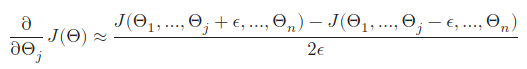
\includegraphics[scale=0.65]{gcmult.png}
    \end{figure}

  \section{Putting it Together}
    First, pick a network architecture; choose the layout of your neural network, including how many hidden units in each layer and how many layers in total you want to have.

    \begin{itemize}
      \item Number of input units = dimension of features $x^{(i)}$
      \item Number of output units = number of classes
      \item Number of hidden units per layer = usually more the better (must balance with the cost of computation as it increases with more hidden units)
      \item Defaults: 1 hidden layer. If you have more than 1 hidden layer, then it is recommended that you have the same number of units in every hidden layer.
    \end{itemize}

    \subsubsection{Training a Neural Network}
      \begin{enumerate}
        \item Randomly initialize the weights\footnote[3]{A good choice for $e_init = \frac{\sqrt{6}}{\sqrt{L_in + L_out}}$}
        \item Implement forward propagation to get $h_\theta(x(i))$ for any $x^{(i)}$
        \item Implement the cost function
        \item Implement backpropagation to compute partial derivatives
        \item Use gradient checking to confirm that your backpropagation works. Then disable gradient checking.
        \item Use gradient descent or a built-in optimization function to minimize the cost function with the weights in theta.
      \end{enumerate}

  % \lstinputlisting[language=octave, caption=Octave implementation for section of Neural Networks]{3.NeuralNetwork.m}

\chapter{Improving Neural Networks}
What to try next for improving our neural networks?
\begin{itemize}
  \item Getting more training examples
  \item Trying smaller sets of features
  \item Trying additional features
  \item Trying polynomial features
  \item Increasing or decreasing $\lambda$
\end{itemize}

\section{Evaulating a Hypothesis}
A hypothesis may have a low error for training examples but still be inaccurate (because of overfitting). Thus, to evaulate a hypothesis, given a dataset of training examples, we can split up the data into two sets: a training set and a test set. Typically, the training set consists of $70\%$ of your data and the test set is the remaining $30\% $.

\begin{figure}[h]
  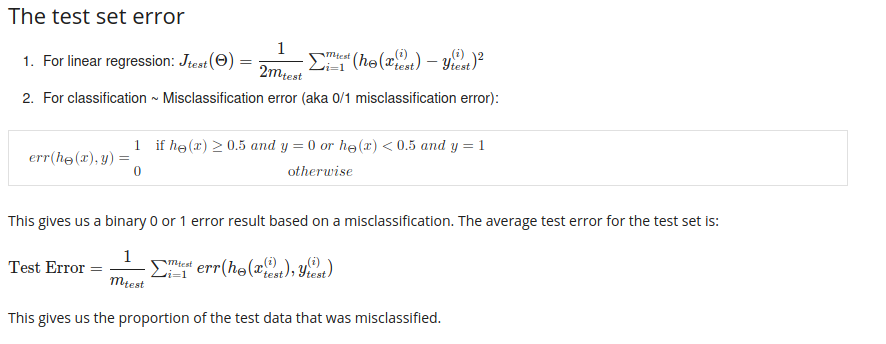
\includegraphics[scale=0.5]{testerror.png}
\end{figure}

\subsection{Model Selection}
  Just because a learning algorithm fits a training set well, that does not mean it is a good hypothesis. It could over fit and as a result your predictions on the test set would be poor.
  \\\\
  Given many models with different polynomial degrees, we can use a systematic approach to identify the 'best' function. In order to choose the model of your hypothesis, you can test each degree of polynomial and look at the error result.
  \\\\
  We usually break down out dataset into three sets:
  \begin{itemize}
    \item Training set: $60\%$
    \item Cross validation set: $20\%$
    \item Test set: $20\%$
  \end{itemize}


  Now to improve our training:
  \begin{enumerate}
    \item Optimize the parameters in $\theta$ using training set.
    \item Find the polynomial degree $d$ with the least error usign the cross validation set.
    \item Estimate the generalization error using the test set with $J_{test}(\Theta^{(d)})$ (d = $\theta$ from polynomial with lower error)
  \end{enumerate}

\section{Bias vs. Variance}
  \textbf{High bias (underfitting)}: both $J_train(\theta)$ and $J_{CV}(\theta)$ will be high and also similar.
  \\\\
  \textbf{High variance (overfitting)}: $J_train(\theta)$ will be low but $J_{CV}(\theta)$.\\

  \begin{figure}[h]
    \centering
    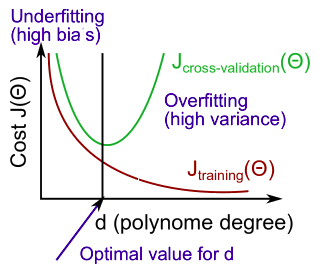
\includegraphics[scale=0.5]{biasVariance.png}
  \end{figure}

  \subsection{Regularization}

    \begin{figure}[h]
      \centering
      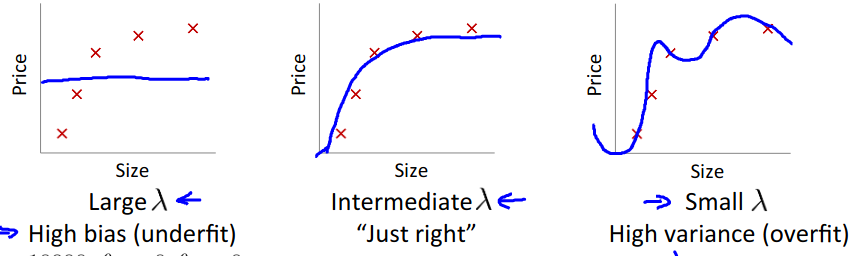
\includegraphics[scale=0.5]{lambda.png}
      \caption{Fitting of data with $\lambda$}
    \end{figure}

    In the figure above, we see that as $\lambda$ increases, our fit becomes more rigid. On the other hand, as $\lambda$ approaches 0, we tend to over overfit the data. So how do we choose our parameter $\lambda$ to get it 'just right' ?

    \begin{enumerate}
      \item Create a list of lambdas.
      \item Iterate through the $\lambda s$ and for each, go throught all the models to learn some $\theta$
      \item Compute the cross validation error.
      \item Select the best combo of $\theta \& \lambda$.
    \end{enumerate}    

  \subsection{Learning Curves}
    \begin{figure}[h]
      \centering
      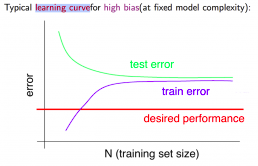
\includegraphics[scale=0.7]{learnbias.png}
      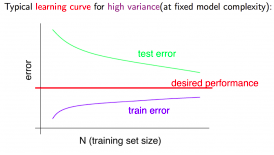
\includegraphics[scale=0.75]{learnvariance.png}
    \end{figure}    
  


\chapter{Unsupervised Learning}
Unsupervised learning is a type of machine learning that looks for previously undetected patterns in a data set with no pre-existing labels and with a minimum of human supervision. In contrast to supervised learning that usually makes use of human-labeled data, unsupervised learning, also known as self-organization allows for modeling of probability densities over inputs. It forms one of the three main categories of machine learning, along with supervised and reinforcement learning. Semi-supervised learning, a related variant, makes use of supervised and unsupervised techniques.

\section{K-Means Clustering Algorithm}
	Kmeans algorithm is an iterative algorithm that tries to partition the dataset into K pre-defined distinct non-overlapping subgroups (clusters) where each data point belongs to only one group. It tries to make the intra-cluster data points as similar as possible while also keeping the clusters as different (far) as possible. It assigns data points to a cluster such that the sum of the squared distance between the data points and the cluster’s centroid (arithmetic mean of all the data points that belong to that cluster) is at the minimum. The less variation we have within clusters, the more homogeneous (similar) the data points are within the same cluster.\\\\

	The way kmeans algorithm works is as follows:
	\begin{enumerate}
		\item Specify number of clusters K.
		\item Initialize centroids by first shuffling the dataset and then randomly selecting K data points for the centroids without replacement.
		\item Keep iterating until there is no change to the centroids. i.e assignment of data points to clusters isn’t changing: 
		\begin{itemize}
			\item Compute the sum of the squared distance between data points and all centroids.
			\item Assign each data point to the closest cluster (centroid).
			\item Compute the centroids for the clusters by taking the average of the all data points that belong to each cluster.
		\end{itemize}
	\end{enumerate}

	\subsection{\textbf{The Elbow Method}: Choosing the number of clusters}
		For the k-means clustering method, the most common approach for choosing the number of clusters is the so-called \textbf{elbow method}. It involves running the algorithm multiple times over a loop, with an increasing number of cluster choice and then plotting a clustering score as a function of the number of clusters.\\

		What is the score or metric which is being plotted for the elbow method? Why is it called the ‘elbow’ method?\\

		A typical plot looks like following,

		\begin{figure}[h]
			\centering
			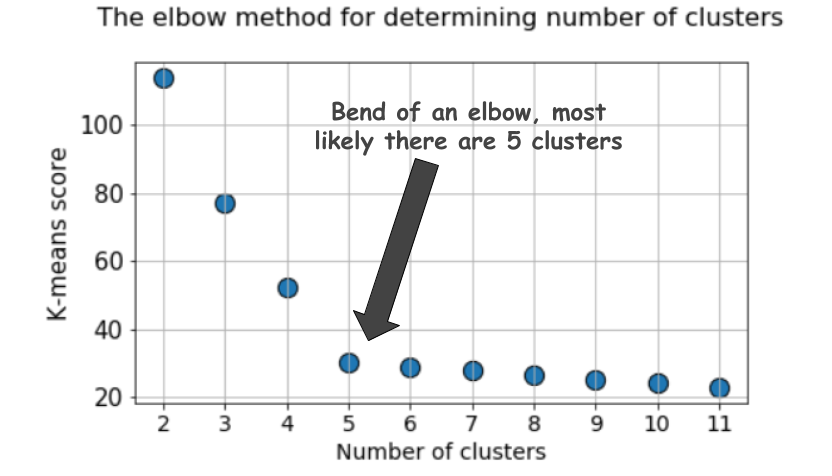
\includegraphics[scale=0.35]{elbow.png}
			\caption{Elbow Method: Score plot}
		\end{figure}

		The score is, in general, a measure of the input data on the k-means objective function i.e. \textbf{some form of intra-cluster distance relative to inner-cluster distance}.


\end{document}